%-------------------------
% Resume in Latex
% Author : Zakaria TOZY
%------------------------

\documentclass[11pt,a4paper]{article}

\usepackage{latexsym}
\usepackage[empty]{fullpage}
\usepackage{titlesec}
\usepackage{marvosym}
\usepackage[usenames,dvipsnames]{color}
\usepackage{verbatim}
\usepackage{enumitem}
\usepackage[hidelinks]{hyperref}
\usepackage{fancyhdr}
\usepackage[english,french]{babel}
\usepackage{tabularx}
\usepackage[utf8]{inputenc}
\usepackage[left=0.5in, right=0.5in, top=0.1in, bottom=0.2in]{geometry}
\usepackage{exscale}  % Pour la commande \HUGE

\usepackage{fontawesome}
\usepackage[scale=0.90,lf]{FiraMono}

\definecolor{light-grey}{gray}{0.83}
\definecolor{dark-grey}{gray}{0.3}
\definecolor{text-grey}{gray}{.08}

\DeclareRobustCommand{\ebseries}{\fontseries{eb}\selectfont}
\DeclareTextFontCommand{\texteb}{\ebseries}

\usepackage{contour}
\usepackage[normalem]{ulem}
\renewcommand{\ULdepth}{1.8pt}
\contourlength{0.8pt}
\newcommand{\myuline}[1]{%
  \uline{\phantom{#1}}%
  \llap{\contour{white}{#1}}%
}

\usepackage{tgheros}
\renewcommand*\familydefault{\sfdefault} 
\usepackage[T1]{fontenc}

\usepackage{graphicx}

\pagestyle{fancy}
\fancyhf{} 
\fancyfoot{}
\renewcommand{\headrulewidth}{0pt}
\renewcommand{\footrulewidth}{0pt}

\urlstyle{same}

\raggedbottom
\raggedright
\setlength{\tabcolsep}{0in}

\titleformat{\section}{
    \bfseries \vspace{-4pt} \raggedright \normalsize
}{}{0em}{}[\color{light-grey} {\titlerule[1pt]} \vspace{-2pt}]

\newcommand{\resumeItem}[1]{
  \item\footnotesize{
    {#1 \vspace{-1pt}}
  }
}

\newcommand{\resumeSubheading}[4]{
  \vspace{2pt}\item
    \begin{tabular*}{\textwidth}[t]{l@{\extracolsep{\fill}}r}
      {\footnotesize\textbf{#1}} & {\footnotesize#2} \\
      {\footnotesize\textit{#3}} & {\footnotesize\textit{#4}} \\
    \end{tabular*}\vspace{2pt}
}

\newcommand{\resumeProjectHeading}[2]{
  \item
  {\footnotesize#1} \hfill {#2}
}

\newcommand{\resumeSubItem}[1]{\resumeItem{#1}\vspace{-4pt}}

\renewcommand\labelitemii{$\vcenter{\hbox{\tiny$\bullet$}}$}

\newcommand{\resumeSubHeadingListStart}{\begin{itemize}[leftmargin=0in, label={}]}
\newcommand{\resumeSubHeadingListEnd}{\end{itemize}}
\newcommand{\resumeItemListStart}{\begin{itemize}[label={\textbullet}]}
\newcommand{\resumeItemListEnd}{\end{itemize}\vspace{0pt}}

\color{text-grey}

\begin{document}

\begin{flushleft}
  \begin{minipage}[c]{0.2\textwidth}
    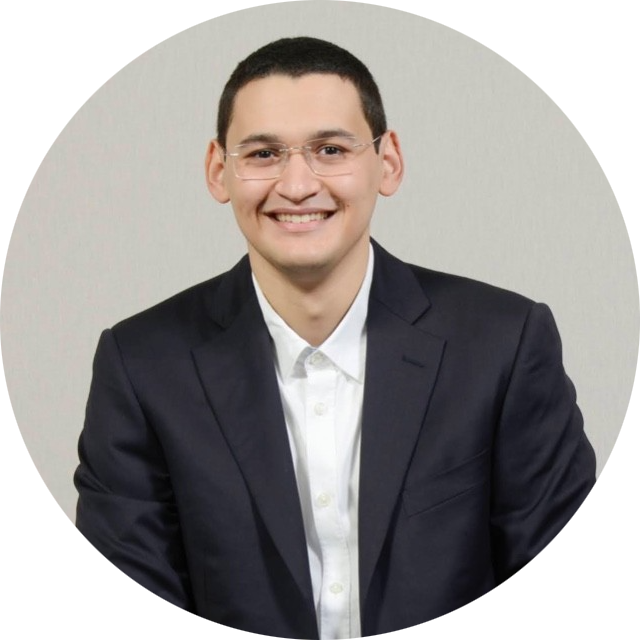
\includegraphics[width=3cm]{images/profilpicture.png}
  \end{minipage}%
  \begin{minipage}[c]{0.8\textwidth}
    {\Huge \textbf{Zakaria TOZY}} \\[5pt]
    {\Large \textbf{Data/ML Engineer | CDI}}
  \end{minipage}
\end{flushleft}

\vspace{-5pt}

\begin{center}
    \small \faPhone\ \texttt{0617407077} \hspace{1pt} $|$
    \hspace{1pt} \faEnvelope\ \texttt{zakaria.tozy@icloud.com} \hspace{1pt} $|$
    \hspace{1pt} \faLinkedin\ \texttt{zakaria-tozy} \hspace{1pt} $|$
    \hspace{1pt} \faMapMarker\ \texttt{Paris} \hspace{1pt} $|$
    \hspace{1pt} \faGithub\ \texttt{github.com/zack242} \\ \vspace{0pt}
\end{center}

\begin{itemize}[leftmargin=0in, label={}]
\footnotesize{\item{
Ingénieur en Data Science avec une double formation (École Polytechnique/ECE Paris), spécialisé en Machine Learning et Data Engineering. Je recherche un poste en CDI pour contribuer à des projets innovants.
}}
\end{itemize}

\section{COMPETENCES}
\begin{itemize}[leftmargin=0in, label={}]
\footnotesize{\item{
{\footnotesize\textbf{Machine Learning}:} {\footnotesize TensorFlow, Scikit-Learn, Deep Learning, NLP} \\
\vspace{3pt}
{\footnotesize\textbf{Cloud}:} {\footnotesize GCP, AWS, Azure, Docker} \\
\vspace{3pt}
{\footnotesize\textbf{Programmation}:} {\footnotesize Python, SQL, Java} \\
\vspace{3pt}
{\footnotesize\textbf{Soft Skills}:} {\footnotesize Autonomie, Rigueur, Esprit d'analyse, Apprentissage rapide} \\
\vspace{3pt}
{\footnotesize\textbf{Langues}:} {\footnotesize Français (Bilingue), Arabe (Bilingue), Anglais (Courant - TOEIC 875)} \\
\vspace{3pt}
{\footnotesize\textbf{Data \& Cloud Engineering}:} {\footnotesize PySpark, Databricks, ETL, Data Pipelines, dbt}
}
}
\end{itemize}

\section{FORMATIONS}
\resumeSubHeadingListStart
    \resumeSubheading
      {Institut Polytechnique de Paris (École Polytechnique)}
      {Janvier 2024}
      {Master 2 en Data Sciences}
      {Mention Très bien}
      \resumeItemListStart
        \resumeItem{Spécialisation : Deep Learning, NLP, Machine Learning, Cloud Computing}
      \resumeItemListEnd
    \resumeSubheading
      {École Centrale d'Électronique (ECE Paris)}
      {Janvier 2024}
      {Ingénieur en Systèmes d'Information et Big Data Analytics}
      {Top 5\% de la promotion}
      \resumeItemListStart
        \resumeItem{Spécialisation : Data Engineering, Machine Learning, Statistiques Avancées}
      \resumeItemListEnd
  \resumeSubHeadingListEnd

\section{EXPERIENCES}
\resumeSubHeadingListStart
    \resumeSubheading
      {AXA Investment Managers - AXA IM}{Août 2023 --- Janvier 2024}
      {Data Engineer/Data Analyst Intern}{Paris}
      \resumeItemListStart
        \resumeItem{Conception et mise en place de pipelines de données sur Databricks pour l'ingestion et la gestion des données métiers}
        \resumeItem{Optimisation du modèle de données et migration des pipelines de distribution}
        \resumeItem{Tests de nouveaux clusters Databricks et création d'un PoC pour l'anonymisation des données}
        \resumeItem{Création de tableaux de bord et calcul des KPIs financiers}
      \resumeItemListEnd
    \resumeSubheading
      {Kalima Blockchain et IoT}{Avril 2022 --- Août 2022}
      {Software Engineer Intern}{Paris}
      \resumeItemListStart
        \resumeItem{Développement d'un explorateur de blockchain propriétaire en Java/LevelDB (1000+ TPS)}
        \resumeItem{Implémentation d'algorithmes d'analyse de données pour le monitoring des transactions}
        \resumeItem{Conception d'un système d'authentification sécurisé}
      \resumeItemListEnd
    \resumeSubheading
      {Le Crédit Lyonnais - LCL}{Janvier 2020 --- Février 2020}
      {IT Intern}{Paris}
      \resumeItemListStart
        \resumeItem{Étude de migration Microsoft Office 2010 vers 2016 et analyse de son impact sur les processus métiers}
        \resumeItem{Développement et exécution de procédures de tests sur un parc de 23 000 postes de travail}
      \resumeItemListEnd
  \resumeSubHeadingListEnd

\section{PROJETS}
\resumeSubHeadingListStart
    \resumeProjectHeading
      {\textbf{Data Challenge \@Natixis}} {}
      \resumeItemListStart
        \resumeItem{Analyse des données textuelles de la FED avec FinBERT dans le but de prédire son impact sur le marché}
      \resumeItemListEnd
    \resumeProjectHeading
      {\textbf{Bitcoin Analysis}} {}
      \resumeItemListStart
        \resumeItem{Pipeline de données (Python, SQL, Airflow, dbt, Snowflake) pour l'analyse de 1M+ transactions Bitcoin par jour}
      \resumeItemListEnd
    \resumeProjectHeading
      {\textbf{Twitter Sentiment Analysis}} {}
      \resumeItemListStart
        \resumeItem{Pipeline temps réel utilisant Kafka et un KNN pour la classification des sentiments en temps réel et en topic}
      \resumeItemListEnd
    \resumeProjectHeading
      {\textbf{Désagrégation de la Courbe Énergétique \@Capgemini}} {}
      \resumeItemListStart
        \resumeItem{Extraction de la composante thermosensible de la consommation énergétique avec un modèle statistique et un réseau de neurones}
      \resumeItemListEnd
\resumeSubHeadingListEnd


\end{document} 